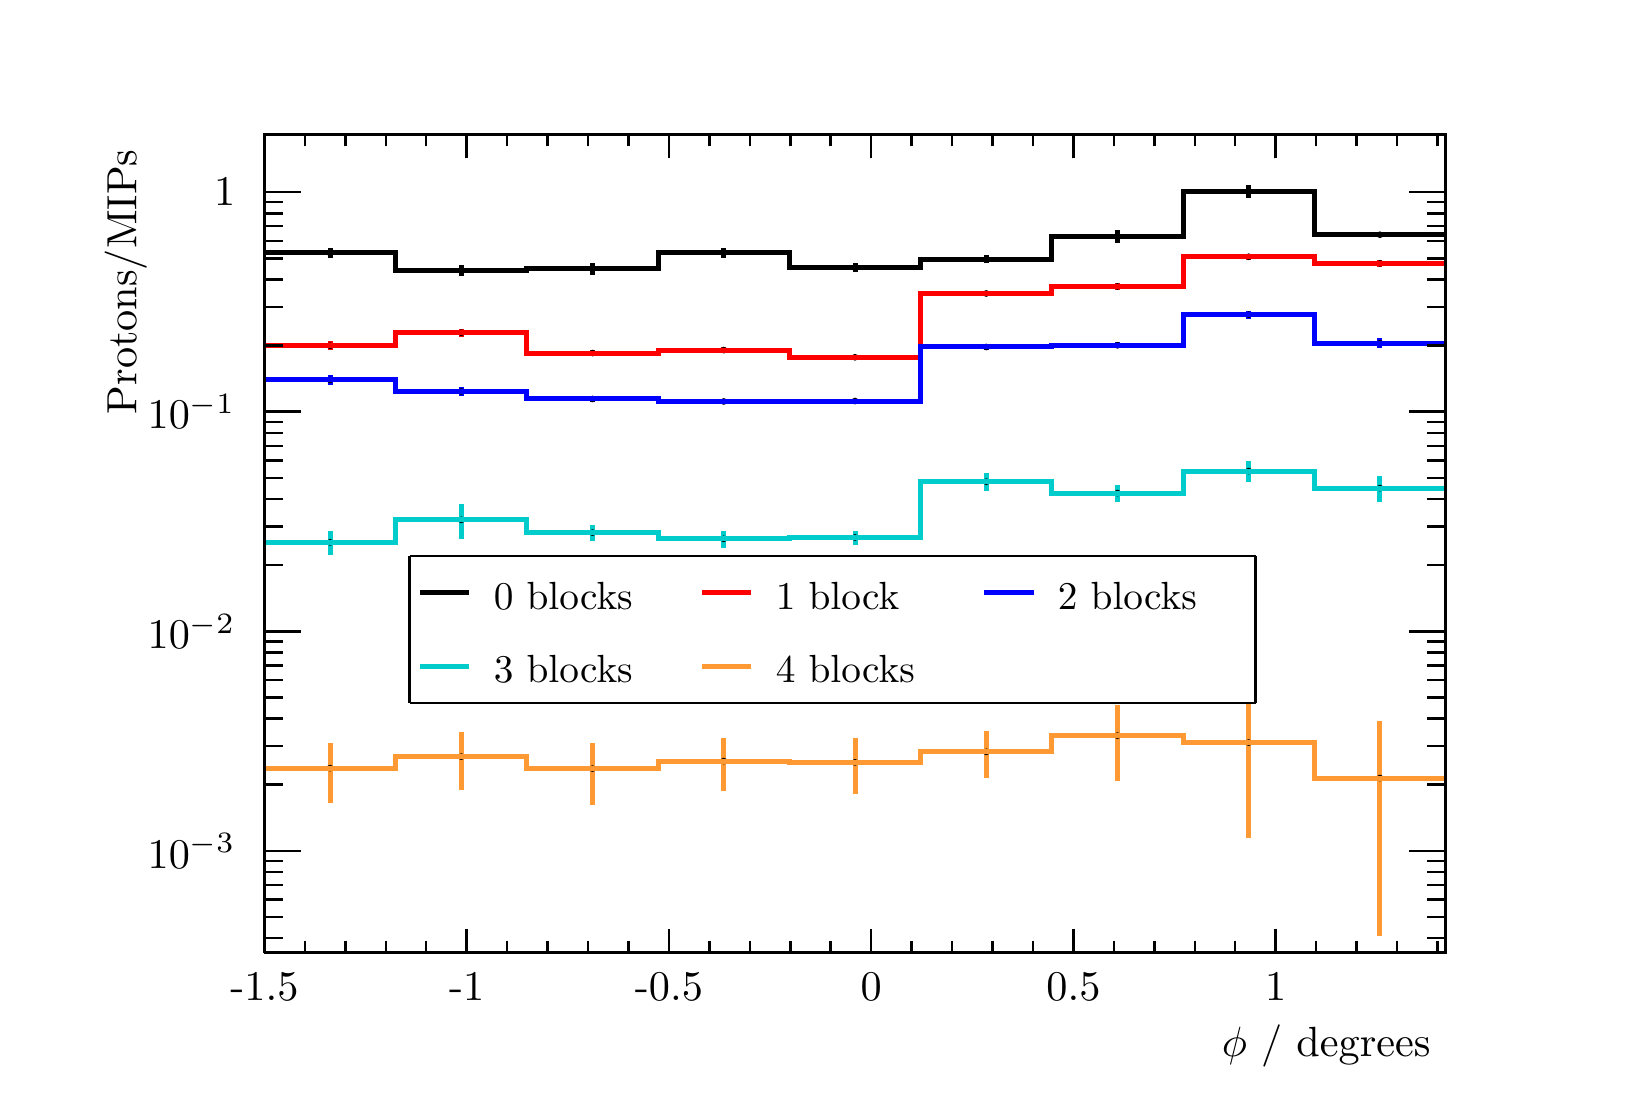
\begin{tikzpicture}
\pgfdeclareplotmark{cross} {
\pgfpathmoveto{\pgfpoint{-0.3\pgfplotmarksize}{\pgfplotmarksize}}
\pgfpathlineto{\pgfpoint{+0.3\pgfplotmarksize}{\pgfplotmarksize}}
\pgfpathlineto{\pgfpoint{+0.3\pgfplotmarksize}{0.3\pgfplotmarksize}}
\pgfpathlineto{\pgfpoint{+1\pgfplotmarksize}{0.3\pgfplotmarksize}}
\pgfpathlineto{\pgfpoint{+1\pgfplotmarksize}{-0.3\pgfplotmarksize}}
\pgfpathlineto{\pgfpoint{+0.3\pgfplotmarksize}{-0.3\pgfplotmarksize}}
\pgfpathlineto{\pgfpoint{+0.3\pgfplotmarksize}{-1.\pgfplotmarksize}}
\pgfpathlineto{\pgfpoint{-0.3\pgfplotmarksize}{-1.\pgfplotmarksize}}
\pgfpathlineto{\pgfpoint{-0.3\pgfplotmarksize}{-0.3\pgfplotmarksize}}
\pgfpathlineto{\pgfpoint{-1.\pgfplotmarksize}{-0.3\pgfplotmarksize}}
\pgfpathlineto{\pgfpoint{-1.\pgfplotmarksize}{0.3\pgfplotmarksize}}
\pgfpathlineto{\pgfpoint{-0.3\pgfplotmarksize}{0.3\pgfplotmarksize}}
\pgfpathclose
\pgfusepathqstroke
}
\pgfdeclareplotmark{cross*} {
\pgfpathmoveto{\pgfpoint{-0.3\pgfplotmarksize}{\pgfplotmarksize}}
\pgfpathlineto{\pgfpoint{+0.3\pgfplotmarksize}{\pgfplotmarksize}}
\pgfpathlineto{\pgfpoint{+0.3\pgfplotmarksize}{0.3\pgfplotmarksize}}
\pgfpathlineto{\pgfpoint{+1\pgfplotmarksize}{0.3\pgfplotmarksize}}
\pgfpathlineto{\pgfpoint{+1\pgfplotmarksize}{-0.3\pgfplotmarksize}}
\pgfpathlineto{\pgfpoint{+0.3\pgfplotmarksize}{-0.3\pgfplotmarksize}}
\pgfpathlineto{\pgfpoint{+0.3\pgfplotmarksize}{-1.\pgfplotmarksize}}
\pgfpathlineto{\pgfpoint{-0.3\pgfplotmarksize}{-1.\pgfplotmarksize}}
\pgfpathlineto{\pgfpoint{-0.3\pgfplotmarksize}{-0.3\pgfplotmarksize}}
\pgfpathlineto{\pgfpoint{-1.\pgfplotmarksize}{-0.3\pgfplotmarksize}}
\pgfpathlineto{\pgfpoint{-1.\pgfplotmarksize}{0.3\pgfplotmarksize}}
\pgfpathlineto{\pgfpoint{-0.3\pgfplotmarksize}{0.3\pgfplotmarksize}}
\pgfpathclose
\pgfusepathqfillstroke
}
\pgfdeclareplotmark{newstar} {
\pgfpathmoveto{\pgfqpoint{0pt}{\pgfplotmarksize}}
\pgfpathlineto{\pgfqpointpolar{44}{0.5\pgfplotmarksize}}
\pgfpathlineto{\pgfqpointpolar{18}{\pgfplotmarksize}}
\pgfpathlineto{\pgfqpointpolar{-20}{0.5\pgfplotmarksize}}
\pgfpathlineto{\pgfqpointpolar{-54}{\pgfplotmarksize}}
\pgfpathlineto{\pgfqpointpolar{-90}{0.5\pgfplotmarksize}}
\pgfpathlineto{\pgfqpointpolar{234}{\pgfplotmarksize}}
\pgfpathlineto{\pgfqpointpolar{198}{0.5\pgfplotmarksize}}
\pgfpathlineto{\pgfqpointpolar{162}{\pgfplotmarksize}}
\pgfpathlineto{\pgfqpointpolar{134}{0.5\pgfplotmarksize}}
\pgfpathclose
\pgfusepathqstroke
}
\pgfdeclareplotmark{newstar*} {
\pgfpathmoveto{\pgfqpoint{0pt}{\pgfplotmarksize}}
\pgfpathlineto{\pgfqpointpolar{44}{0.5\pgfplotmarksize}}
\pgfpathlineto{\pgfqpointpolar{18}{\pgfplotmarksize}}
\pgfpathlineto{\pgfqpointpolar{-20}{0.5\pgfplotmarksize}}
\pgfpathlineto{\pgfqpointpolar{-54}{\pgfplotmarksize}}
\pgfpathlineto{\pgfqpointpolar{-90}{0.5\pgfplotmarksize}}
\pgfpathlineto{\pgfqpointpolar{234}{\pgfplotmarksize}}
\pgfpathlineto{\pgfqpointpolar{198}{0.5\pgfplotmarksize}}
\pgfpathlineto{\pgfqpointpolar{162}{\pgfplotmarksize}}
\pgfpathlineto{\pgfqpointpolar{134}{0.5\pgfplotmarksize}}
\pgfpathclose
\pgfusepathqfillstroke
}
\definecolor{c}{rgb}{1,1,1};
\draw [color=c, fill=c] (0,0) rectangle (20,13.4957);
\draw [color=c, fill=c] (3,1.75444) rectangle (18,12.1461);
\definecolor{c}{rgb}{0,0,0};
\draw [c,line width=0.9] (3,1.75444) -- (3,12.1461) -- (18,12.1461) -- (18,1.75444) -- (3,1.75444);
\definecolor{c}{rgb}{1,1,1};
\draw [color=c, fill=c] (3,1.75444) rectangle (18,12.1461);
\definecolor{c}{rgb}{0,0,0};
\draw [c,line width=0.9] (3,1.75444) -- (3,12.1461) -- (18,12.1461) -- (18,1.75444) -- (3,1.75444);
\draw [c,line width=0.9] (3,1.75444) -- (4.66667,1.75444) -- (4.66667,1.75444) -- (6.33333,1.75444) -- (6.33333,1.75444) -- (8,1.75444) -- (8,1.75444) -- (9.66667,1.75444) -- (9.66667,1.75444) -- (11.3333,1.75444) -- (11.3333,1.75444) -- (13,1.75444)
 -- (13,1.75444) -- (14.6667,1.75444) -- (14.6667,1.75444) -- (16.3333,1.75444) -- (16.3333,1.75444) -- (18,1.75444);
\draw [c,line width=0.9] (3,1.75444) -- (18,1.75444);
\draw [c,line width=0.9] (3,2.05809) -- (3,1.75444);
\draw [c,line width=0.9] (3.5137,1.90627) -- (3.5137,1.75444);
\draw [c,line width=0.9] (4.0274,1.90627) -- (4.0274,1.75444);
\draw [c,line width=0.9] (4.5411,1.90627) -- (4.5411,1.75444);
\draw [c,line width=0.9] (5.05479,1.90627) -- (5.05479,1.75444);
\draw [c,line width=0.9] (5.56849,2.05809) -- (5.56849,1.75444);
\draw [c,line width=0.9] (6.08219,1.90627) -- (6.08219,1.75444);
\draw [c,line width=0.9] (6.59589,1.90627) -- (6.59589,1.75444);
\draw [c,line width=0.9] (7.10959,1.90627) -- (7.10959,1.75444);
\draw [c,line width=0.9] (7.62329,1.90627) -- (7.62329,1.75444);
\draw [c,line width=0.9] (8.13699,2.05809) -- (8.13699,1.75444);
\draw [c,line width=0.9] (8.65069,1.90627) -- (8.65069,1.75444);
\draw [c,line width=0.9] (9.16438,1.90627) -- (9.16438,1.75444);
\draw [c,line width=0.9] (9.67808,1.90627) -- (9.67808,1.75444);
\draw [c,line width=0.9] (10.1918,1.90627) -- (10.1918,1.75444);
\draw [c,line width=0.9] (10.7055,2.05809) -- (10.7055,1.75444);
\draw [c,line width=0.9] (11.2192,1.90627) -- (11.2192,1.75444);
\draw [c,line width=0.9] (11.7329,1.90627) -- (11.7329,1.75444);
\draw [c,line width=0.9] (12.2466,1.90627) -- (12.2466,1.75444);
\draw [c,line width=0.9] (12.7603,1.90627) -- (12.7603,1.75444);
\draw [c,line width=0.9] (13.274,2.05809) -- (13.274,1.75444);
\draw [c,line width=0.9] (13.7877,1.90627) -- (13.7877,1.75444);
\draw [c,line width=0.9] (14.3014,1.90627) -- (14.3014,1.75444);
\draw [c,line width=0.9] (14.8151,1.90627) -- (14.8151,1.75444);
\draw [c,line width=0.9] (15.3288,1.90627) -- (15.3288,1.75444);
\draw [c,line width=0.9] (15.8425,2.05809) -- (15.8425,1.75444);
\draw [c,line width=0.9] (15.8425,2.05809) -- (15.8425,1.75444);
\draw [c,line width=0.9] (16.3562,1.90627) -- (16.3562,1.75444);
\draw [c,line width=0.9] (16.8699,1.90627) -- (16.8699,1.75444);
\draw [c,line width=0.9] (17.3836,1.90627) -- (17.3836,1.75444);
\draw [c,line width=0.9] (17.8973,1.90627) -- (17.8973,1.75444);
\draw [anchor=base] (3,1.14713) node[scale=1.52731, color=c, rotate=0]{-1.5};
\draw [anchor=base] (5.56849,1.14713) node[scale=1.52731, color=c, rotate=0]{-1};
\draw [anchor=base] (8.13699,1.14713) node[scale=1.52731, color=c, rotate=0]{-0.5};
\draw [anchor=base] (10.7055,1.14713) node[scale=1.52731, color=c, rotate=0]{0};
\draw [anchor=base] (13.274,1.14713) node[scale=1.52731, color=c, rotate=0]{0.5};
\draw [anchor=base] (15.8425,1.14713) node[scale=1.52731, color=c, rotate=0]{1};
\draw [anchor= east] (18,0.566819) node[scale=1.52731, color=c, rotate=0]{$ \phi$ / degrees};
\draw [c,line width=0.9] (3,12.1461) -- (18,12.1461);
\draw [c,line width=0.9] (3,11.8425) -- (3,12.1461);
\draw [c,line width=0.9] (3.5137,11.9943) -- (3.5137,12.1461);
\draw [c,line width=0.9] (4.0274,11.9943) -- (4.0274,12.1461);
\draw [c,line width=0.9] (4.5411,11.9943) -- (4.5411,12.1461);
\draw [c,line width=0.9] (5.05479,11.9943) -- (5.05479,12.1461);
\draw [c,line width=0.9] (5.56849,11.8425) -- (5.56849,12.1461);
\draw [c,line width=0.9] (6.08219,11.9943) -- (6.08219,12.1461);
\draw [c,line width=0.9] (6.59589,11.9943) -- (6.59589,12.1461);
\draw [c,line width=0.9] (7.10959,11.9943) -- (7.10959,12.1461);
\draw [c,line width=0.9] (7.62329,11.9943) -- (7.62329,12.1461);
\draw [c,line width=0.9] (8.13699,11.8425) -- (8.13699,12.1461);
\draw [c,line width=0.9] (8.65069,11.9943) -- (8.65069,12.1461);
\draw [c,line width=0.9] (9.16438,11.9943) -- (9.16438,12.1461);
\draw [c,line width=0.9] (9.67808,11.9943) -- (9.67808,12.1461);
\draw [c,line width=0.9] (10.1918,11.9943) -- (10.1918,12.1461);
\draw [c,line width=0.9] (10.7055,11.8425) -- (10.7055,12.1461);
\draw [c,line width=0.9] (11.2192,11.9943) -- (11.2192,12.1461);
\draw [c,line width=0.9] (11.7329,11.9943) -- (11.7329,12.1461);
\draw [c,line width=0.9] (12.2466,11.9943) -- (12.2466,12.1461);
\draw [c,line width=0.9] (12.7603,11.9943) -- (12.7603,12.1461);
\draw [c,line width=0.9] (13.274,11.8425) -- (13.274,12.1461);
\draw [c,line width=0.9] (13.7877,11.9943) -- (13.7877,12.1461);
\draw [c,line width=0.9] (14.3014,11.9943) -- (14.3014,12.1461);
\draw [c,line width=0.9] (14.8151,11.9943) -- (14.8151,12.1461);
\draw [c,line width=0.9] (15.3288,11.9943) -- (15.3288,12.1461);
\draw [c,line width=0.9] (15.8425,11.8425) -- (15.8425,12.1461);
\draw [c,line width=0.9] (15.8425,11.8425) -- (15.8425,12.1461);
\draw [c,line width=0.9] (16.3562,11.9943) -- (16.3562,12.1461);
\draw [c,line width=0.9] (16.8699,11.9943) -- (16.8699,12.1461);
\draw [c,line width=0.9] (17.3836,11.9943) -- (17.3836,12.1461);
\draw [c,line width=0.9] (17.8973,11.9943) -- (17.8973,12.1461);
\draw [c,line width=0.9] (3,1.75444) -- (3,12.1461);
\draw [c,line width=0.9] (3.231,1.93919) -- (3,1.93919);
\draw [c,line width=0.9] (3.231,2.20939) -- (3,2.20939);
\draw [c,line width=0.9] (3.231,2.43016) -- (3,2.43016);
\draw [c,line width=0.9] (3.231,2.61681) -- (3,2.61681);
\draw [c,line width=0.9] (3.231,2.7785) -- (3,2.7785);
\draw [c,line width=0.9] (3.231,2.92112) -- (3,2.92112);
\draw [c,line width=0.9] (3.462,3.0487) -- (3,3.0487);
\draw [anchor= east] (2.82,3.0487) node[scale=1.52731, color=c, rotate=0]{$10^{-3}$};
\draw [c,line width=0.9] (3.231,3.88801) -- (3,3.88801);
\draw [c,line width=0.9] (3.231,4.37898) -- (3,4.37898);
\draw [c,line width=0.9] (3.231,4.72732) -- (3,4.72732);
\draw [c,line width=0.9] (3.231,4.99752) -- (3,4.99752);
\draw [c,line width=0.9] (3.231,5.21829) -- (3,5.21829);
\draw [c,line width=0.9] (3.231,5.40494) -- (3,5.40494);
\draw [c,line width=0.9] (3.231,5.56663) -- (3,5.56663);
\draw [c,line width=0.9] (3.231,5.70925) -- (3,5.70925);
\draw [c,line width=0.9] (3.462,5.83683) -- (3,5.83683);
\draw [anchor= east] (2.82,5.83683) node[scale=1.52731, color=c, rotate=0]{$10^{-2}$};
\draw [c,line width=0.9] (3.231,6.67614) -- (3,6.67614);
\draw [c,line width=0.9] (3.231,7.16711) -- (3,7.16711);
\draw [c,line width=0.9] (3.231,7.51545) -- (3,7.51545);
\draw [c,line width=0.9] (3.231,7.78565) -- (3,7.78565);
\draw [c,line width=0.9] (3.231,8.00642) -- (3,8.00642);
\draw [c,line width=0.9] (3.231,8.19307) -- (3,8.19307);
\draw [c,line width=0.9] (3.231,8.35476) -- (3,8.35476);
\draw [c,line width=0.9] (3.231,8.49738) -- (3,8.49738);
\draw [c,line width=0.9] (3.462,8.62496) -- (3,8.62496);
\draw [anchor= east] (2.82,8.62496) node[scale=1.52731, color=c, rotate=0]{$10^{-1}$};
\draw [c,line width=0.9] (3.231,9.46427) -- (3,9.46427);
\draw [c,line width=0.9] (3.231,9.95524) -- (3,9.95524);
\draw [c,line width=0.9] (3.231,10.3036) -- (3,10.3036);
\draw [c,line width=0.9] (3.231,10.5738) -- (3,10.5738);
\draw [c,line width=0.9] (3.231,10.7945) -- (3,10.7945);
\draw [c,line width=0.9] (3.231,10.9812) -- (3,10.9812);
\draw [c,line width=0.9] (3.231,11.1429) -- (3,11.1429);
\draw [c,line width=0.9] (3.231,11.2855) -- (3,11.2855);
\draw [c,line width=0.9] (3.462,11.4131) -- (3,11.4131);
\draw [anchor= east] (2.82,11.4131) node[scale=1.52731, color=c, rotate=0]{1};
\draw [anchor= east] (1.24,12.1461) node[scale=1.52731, color=c, rotate=90]{ Protons/MIPs};
\draw [c,line width=0.9] (18,1.75444) -- (18,12.1461);
\draw [c,line width=0.9] (17.769,1.93919) -- (18,1.93919);
\draw [c,line width=0.9] (17.769,2.20939) -- (18,2.20939);
\draw [c,line width=0.9] (17.769,2.43016) -- (18,2.43016);
\draw [c,line width=0.9] (17.769,2.61681) -- (18,2.61681);
\draw [c,line width=0.9] (17.769,2.7785) -- (18,2.7785);
\draw [c,line width=0.9] (17.769,2.92112) -- (18,2.92112);
\draw [c,line width=0.9] (17.538,3.0487) -- (18,3.0487);
\draw [c,line width=0.9] (17.769,3.88801) -- (18,3.88801);
\draw [c,line width=0.9] (17.769,4.37898) -- (18,4.37898);
\draw [c,line width=0.9] (17.769,4.72732) -- (18,4.72732);
\draw [c,line width=0.9] (17.769,4.99752) -- (18,4.99752);
\draw [c,line width=0.9] (17.769,5.21829) -- (18,5.21829);
\draw [c,line width=0.9] (17.769,5.40494) -- (18,5.40494);
\draw [c,line width=0.9] (17.769,5.56663) -- (18,5.56663);
\draw [c,line width=0.9] (17.769,5.70925) -- (18,5.70925);
\draw [c,line width=0.9] (17.538,5.83683) -- (18,5.83683);
\draw [c,line width=0.9] (17.769,6.67614) -- (18,6.67614);
\draw [c,line width=0.9] (17.769,7.16711) -- (18,7.16711);
\draw [c,line width=0.9] (17.769,7.51545) -- (18,7.51545);
\draw [c,line width=0.9] (17.769,7.78565) -- (18,7.78565);
\draw [c,line width=0.9] (17.769,8.00642) -- (18,8.00642);
\draw [c,line width=0.9] (17.769,8.19307) -- (18,8.19307);
\draw [c,line width=0.9] (17.769,8.35476) -- (18,8.35476);
\draw [c,line width=0.9] (17.769,8.49738) -- (18,8.49738);
\draw [c,line width=0.9] (17.538,8.62496) -- (18,8.62496);
\draw [c,line width=0.9] (17.769,9.46427) -- (18,9.46427);
\draw [c,line width=0.9] (17.769,9.95524) -- (18,9.95524);
\draw [c,line width=0.9] (17.769,10.3036) -- (18,10.3036);
\draw [c,line width=0.9] (17.769,10.5738) -- (18,10.5738);
\draw [c,line width=0.9] (17.769,10.7945) -- (18,10.7945);
\draw [c,line width=0.9] (17.769,10.9812) -- (18,10.9812);
\draw [c,line width=0.9] (17.769,11.1429) -- (18,11.1429);
\draw [c,line width=0.9] (17.769,11.2855) -- (18,11.2855);
\draw [c,line width=0.9] (17.538,11.4131) -- (18,11.4131);
\draw [c,line width=1.8] (3.83333,10.572) -- (3.83333,10.6419);
\draw [c,line width=1.8] (3.83333,10.6419) -- (3.83333,10.7081);
\foreach \P in {(3.83333,10.6419)}{\draw[mark options={color=c,fill=c},mark size=2.402402pt,mark=*,mark size=1pt] plot coordinates {\P};}
\draw [c,line width=1.8] (5.5,10.3482) -- (5.5,10.42);
\draw [c,line width=1.8] (5.5,10.42) -- (5.5,10.4878);
\foreach \P in {(5.5,10.42)}{\draw[mark options={color=c,fill=c},mark size=2.402402pt,mark=*,mark size=1pt] plot coordinates {\P};}
\draw [c,line width=1.8] (7.16667,10.3597) -- (7.16667,10.4384);
\draw [c,line width=1.8] (7.16667,10.4384) -- (7.16667,10.5124);
\foreach \P in {(7.16667,10.4384)}{\draw[mark options={color=c,fill=c},mark size=2.402402pt,mark=*,mark size=1pt] plot coordinates {\P};}
\draw [c,line width=1.8] (8.83333,10.5821) -- (8.83333,10.6443);
\draw [c,line width=1.8] (8.83333,10.6443) -- (8.83333,10.7033);
\foreach \P in {(8.83333,10.6443)}{\draw[mark options={color=c,fill=c},mark size=2.402402pt,mark=*,mark size=1pt] plot coordinates {\P};}
\draw [c,line width=1.8] (10.5,10.3955) -- (10.5,10.4552);
\draw [c,line width=1.8] (10.5,10.4552) -- (10.5,10.5121);
\foreach \P in {(10.5,10.4552)}{\draw[mark options={color=c,fill=c},mark size=2.402402pt,mark=*,mark size=1pt] plot coordinates {\P};}
\draw [c,line width=1.8] (12.1667,10.5095) -- (12.1667,10.5604);
\draw [c,line width=1.8] (12.1667,10.5604) -- (12.1667,10.6093);
\foreach \P in {(12.1667,10.5604)}{\draw[mark options={color=c,fill=c},mark size=2.402402pt,mark=*,mark size=1pt] plot coordinates {\P};}
\draw [c,line width=1.8] (13.8333,10.7682) -- (13.8333,10.8531);
\draw [c,line width=1.8] (13.8333,10.8531) -- (13.8333,10.9325);
\foreach \P in {(13.8333,10.8531)}{\draw[mark options={color=c,fill=c},mark size=2.402402pt,mark=*,mark size=1pt] plot coordinates {\P};}
\draw [c,line width=1.8] (15.5,11.3373) -- (15.5,11.424);
\draw [c,line width=1.8] (15.5,11.424) -- (15.5,11.505);
\foreach \P in {(15.5,11.424)}{\draw[mark options={color=c,fill=c},mark size=2.402402pt,mark=*,mark size=1pt] plot coordinates {\P};}
\draw [c,line width=1.8] (17.1667,10.8476) -- (17.1667,10.8726);
\draw [c,line width=1.8] (17.1667,10.8726) -- (17.1667,10.8972);
\foreach \P in {(17.1667,10.8726)}{\draw[mark options={color=c,fill=c},mark size=2.402402pt,mark=*,mark size=1pt] plot coordinates {\P};}
\draw [c,line width=1.8] (3,10.6419) -- (4.66667,10.6419) -- (4.66667,10.42) -- (6.33333,10.42) -- (6.33333,10.4384) -- (8,10.4384) -- (8,10.6443) -- (9.66667,10.6443) -- (9.66667,10.4552) -- (11.3333,10.4552) -- (11.3333,10.5604) -- (13,10.5604) --
 (13,10.8531) -- (14.6667,10.8531) -- (14.6667,11.424) -- (16.3333,11.424) -- (16.3333,10.8726) -- (18,10.8726);
\definecolor{c}{rgb}{1,0,0};
\draw [c,line width=1.8] (3.83333,9.40359) -- (3.83333,9.46301);
\draw [c,line width=1.8] (3.83333,9.46301) -- (3.83333,9.51965);
\definecolor{c}{rgb}{0,0,0};
\foreach \P in {(3.83333,9.46301)}{\draw[mark options={color=c,fill=c},mark size=2.402402pt,mark=*,mark size=1pt] plot coordinates {\P};}
\definecolor{c}{rgb}{1,0,0};
\draw [c,line width=1.8] (5.5,9.57854) -- (5.5,9.62851);
\draw [c,line width=1.8] (5.5,9.62851) -- (5.5,9.6765);
\definecolor{c}{rgb}{0,0,0};
\foreach \P in {(5.5,9.62851)}{\draw[mark options={color=c,fill=c},mark size=2.402402pt,mark=*,mark size=1pt] plot coordinates {\P};}
\definecolor{c}{rgb}{1,0,0};
\draw [c,line width=1.8] (7.16667,9.33523) -- (7.16667,9.37043);
\draw [c,line width=1.8] (7.16667,9.37043) -- (7.16667,9.40463);
\definecolor{c}{rgb}{0,0,0};
\foreach \P in {(7.16667,9.37043)}{\draw[mark options={color=c,fill=c},mark size=2.402402pt,mark=*,mark size=1pt] plot coordinates {\P};}
\definecolor{c}{rgb}{1,0,0};
\draw [c,line width=1.8] (8.83333,9.37028) -- (8.83333,9.40777);
\draw [c,line width=1.8] (8.83333,9.40777) -- (8.83333,9.44414);
\definecolor{c}{rgb}{0,0,0};
\foreach \P in {(8.83333,9.40777)}{\draw[mark options={color=c,fill=c},mark size=2.402402pt,mark=*,mark size=1pt] plot coordinates {\P};}
\definecolor{c}{rgb}{1,0,0};
\draw [c,line width=1.8] (10.5,9.28506) -- (10.5,9.31673);
\draw [c,line width=1.8] (10.5,9.31673) -- (10.5,9.3476);
\definecolor{c}{rgb}{0,0,0};
\foreach \P in {(10.5,9.31673)}{\draw[mark options={color=c,fill=c},mark size=2.402402pt,mark=*,mark size=1pt] plot coordinates {\P};}
\definecolor{c}{rgb}{1,0,0};
\draw [c,line width=1.8] (12.1667,10.0925) -- (12.1667,10.1267);
\draw [c,line width=1.8] (12.1667,10.1267) -- (12.1667,10.1601);
\definecolor{c}{rgb}{0,0,0};
\foreach \P in {(12.1667,10.1267)}{\draw[mark options={color=c,fill=c},mark size=2.402402pt,mark=*,mark size=1pt] plot coordinates {\P};}
\definecolor{c}{rgb}{1,0,0};
\draw [c,line width=1.8] (13.8333,10.1698) -- (13.8333,10.2162);
\draw [c,line width=1.8] (13.8333,10.2162) -- (13.8333,10.261);
\definecolor{c}{rgb}{0,0,0};
\foreach \P in {(13.8333,10.2162)}{\draw[mark options={color=c,fill=c},mark size=2.402402pt,mark=*,mark size=1pt] plot coordinates {\P};}
\definecolor{c}{rgb}{1,0,0};
\draw [c,line width=1.8] (15.5,10.5564) -- (15.5,10.5934);
\draw [c,line width=1.8] (15.5,10.5934) -- (15.5,10.6294);
\definecolor{c}{rgb}{0,0,0};
\foreach \P in {(15.5,10.5934)}{\draw[mark options={color=c,fill=c},mark size=2.402402pt,mark=*,mark size=1pt] plot coordinates {\P};}
\definecolor{c}{rgb}{1,0,0};
\draw [c,line width=1.8] (17.1667,10.4672) -- (17.1667,10.5099);
\draw [c,line width=1.8] (17.1667,10.5099) -- (17.1667,10.5512);
\definecolor{c}{rgb}{0,0,0};
\foreach \P in {(17.1667,10.5099)}{\draw[mark options={color=c,fill=c},mark size=2.402402pt,mark=*,mark size=1pt] plot coordinates {\P};}
\definecolor{c}{rgb}{1,0,0};
\draw [c,line width=1.8] (3,9.46301) -- (4.66667,9.46301) -- (4.66667,9.62851) -- (6.33333,9.62851) -- (6.33333,9.37043) -- (8,9.37043) -- (8,9.40777) -- (9.66667,9.40777) -- (9.66667,9.31673) -- (11.3333,9.31673) -- (11.3333,10.1267) -- (13,10.1267)
 -- (13,10.2162) -- (14.6667,10.2162) -- (14.6667,10.5934) -- (16.3333,10.5934) -- (16.3333,10.5099) -- (18,10.5099);
\definecolor{c}{rgb}{0,0,1};
\draw [c,line width=1.8] (3.83333,8.96981) -- (3.83333,9.02932);
\draw [c,line width=1.8] (3.83333,9.02932) -- (3.83333,9.08605);
\definecolor{c}{rgb}{0,0,0};
\foreach \P in {(3.83333,9.02932)}{\draw[mark options={color=c,fill=c},mark size=2.402402pt,mark=*,mark size=1pt] plot coordinates {\P};}
\definecolor{c}{rgb}{0,0,1};
\draw [c,line width=1.8] (5.5,8.83028) -- (5.5,8.88269);
\draw [c,line width=1.8] (5.5,8.88269) -- (5.5,8.93294);
\definecolor{c}{rgb}{0,0,0};
\foreach \P in {(5.5,8.88269)}{\draw[mark options={color=c,fill=c},mark size=2.402402pt,mark=*,mark size=1pt] plot coordinates {\P};}
\definecolor{c}{rgb}{0,0,1};
\draw [c,line width=1.8] (7.16667,8.74754) -- (7.16667,8.78715);
\draw [c,line width=1.8] (7.16667,8.78715) -- (7.16667,8.82551);
\definecolor{c}{rgb}{0,0,0};
\foreach \P in {(7.16667,8.78715)}{\draw[mark options={color=c,fill=c},mark size=2.402402pt,mark=*,mark size=1pt] plot coordinates {\P};}
\definecolor{c}{rgb}{0,0,1};
\draw [c,line width=1.8] (8.83333,8.72092) -- (8.83333,8.75543);
\draw [c,line width=1.8] (8.83333,8.75543) -- (8.83333,8.78898);
\definecolor{c}{rgb}{0,0,0};
\foreach \P in {(8.83333,8.75543)}{\draw[mark options={color=c,fill=c},mark size=2.402402pt,mark=*,mark size=1pt] plot coordinates {\P};}
\definecolor{c}{rgb}{0,0,1};
\draw [c,line width=1.8] (10.5,8.73099) -- (10.5,8.76081);
\draw [c,line width=1.8] (10.5,8.76081) -- (10.5,8.78991);
\definecolor{c}{rgb}{0,0,0};
\foreach \P in {(10.5,8.76081)}{\draw[mark options={color=c,fill=c},mark size=2.402402pt,mark=*,mark size=1pt] plot coordinates {\P};}
\definecolor{c}{rgb}{0,0,1};
\draw [c,line width=1.8] (12.1667,9.41213) -- (12.1667,9.44762);
\draw [c,line width=1.8] (12.1667,9.44762) -- (12.1667,9.48209);
\definecolor{c}{rgb}{0,0,0};
\foreach \P in {(12.1667,9.44762)}{\draw[mark options={color=c,fill=c},mark size=2.402402pt,mark=*,mark size=1pt] plot coordinates {\P};}
\definecolor{c}{rgb}{0,0,1};
\draw [c,line width=1.8] (13.8333,9.43055) -- (13.8333,9.4684);
\draw [c,line width=1.8] (13.8333,9.4684) -- (13.8333,9.5051);
\definecolor{c}{rgb}{0,0,0};
\foreach \P in {(13.8333,9.4684)}{\draw[mark options={color=c,fill=c},mark size=2.402402pt,mark=*,mark size=1pt] plot coordinates {\P};}
\definecolor{c}{rgb}{0,0,1};
\draw [c,line width=1.8] (15.5,9.80824) -- (15.5,9.8583);
\draw [c,line width=1.8] (15.5,9.8583) -- (15.5,9.90637);
\definecolor{c}{rgb}{0,0,0};
\foreach \P in {(15.5,9.8583)}{\draw[mark options={color=c,fill=c},mark size=2.402402pt,mark=*,mark size=1pt] plot coordinates {\P};}
\definecolor{c}{rgb}{0,0,1};
\draw [c,line width=1.8] (17.1667,9.43336) -- (17.1667,9.49632);
\draw [c,line width=1.8] (17.1667,9.49632) -- (17.1667,9.55617);
\definecolor{c}{rgb}{0,0,0};
\foreach \P in {(17.1667,9.49632)}{\draw[mark options={color=c,fill=c},mark size=2.402402pt,mark=*,mark size=1pt] plot coordinates {\P};}
\definecolor{c}{rgb}{0,0,1};
\draw [c,line width=1.8] (3,9.02932) -- (4.66667,9.02932) -- (4.66667,8.88269) -- (6.33333,8.88269) -- (6.33333,8.78715) -- (8,8.78715) -- (8,8.75543) -- (9.66667,8.75543) -- (9.66667,8.76081) -- (11.3333,8.76081) -- (11.3333,9.44762) -- (13,9.44762)
 -- (13,9.4684) -- (14.6667,9.4684) -- (14.6667,9.8583) -- (16.3333,9.8583) -- (16.3333,9.49632) -- (18,9.49632);
\definecolor{c}{rgb}{0,0.8,0.8};
\draw [c,line width=1.8] (3.83333,6.80707) -- (3.83333,6.96591);
\draw [c,line width=1.8] (3.83333,6.96591) -- (3.83333,7.10631);
\definecolor{c}{rgb}{0,0,0};
\foreach \P in {(3.83333,6.96591)}{\draw[mark options={color=c,fill=c},mark size=2.402402pt,mark=*,mark size=1pt] plot coordinates {\P};}
\definecolor{c}{rgb}{0,0.8,0.8};
\draw [c,line width=1.8] (5.5,7.00316) -- (5.5,7.25221);
\draw [c,line width=1.8] (5.5,7.25221) -- (5.5,7.45867);
\definecolor{c}{rgb}{0,0,0};
\foreach \P in {(5.5,7.25221)}{\draw[mark options={color=c,fill=c},mark size=2.402402pt,mark=*,mark size=1pt] plot coordinates {\P};}
\definecolor{c}{rgb}{0,0.8,0.8};
\draw [c,line width=1.8] (7.16667,6.97812) -- (7.16667,7.08972);
\draw [c,line width=1.8] (7.16667,7.08972) -- (7.16667,7.1919);
\definecolor{c}{rgb}{0,0,0};
\foreach \P in {(7.16667,7.08972)}{\draw[mark options={color=c,fill=c},mark size=2.402402pt,mark=*,mark size=1pt] plot coordinates {\P};}
\definecolor{c}{rgb}{0,0.8,0.8};
\draw [c,line width=1.8] (8.83333,6.89753) -- (8.83333,7.01091);
\draw [c,line width=1.8] (8.83333,7.01091) -- (8.83333,7.11458);
\definecolor{c}{rgb}{0,0,0};
\foreach \P in {(8.83333,7.01091)}{\draw[mark options={color=c,fill=c},mark size=2.402402pt,mark=*,mark size=1pt] plot coordinates {\P};}
\definecolor{c}{rgb}{0,0.8,0.8};
\draw [c,line width=1.8] (10.5,6.9388) -- (10.5,7.0284);
\draw [c,line width=1.8] (10.5,7.0284) -- (10.5,7.11182);
\definecolor{c}{rgb}{0,0,0};
\foreach \P in {(10.5,7.0284)}{\draw[mark options={color=c,fill=c},mark size=2.402402pt,mark=*,mark size=1pt] plot coordinates {\P};}
\definecolor{c}{rgb}{0,0.8,0.8};
\draw [c,line width=1.8] (12.1667,7.61534) -- (12.1667,7.73673);
\draw [c,line width=1.8] (12.1667,7.73673) -- (12.1667,7.84705);
\definecolor{c}{rgb}{0,0,0};
\foreach \P in {(12.1667,7.73673)}{\draw[mark options={color=c,fill=c},mark size=2.402402pt,mark=*,mark size=1pt] plot coordinates {\P};}
\definecolor{c}{rgb}{0,0.8,0.8};
\draw [c,line width=1.8] (13.8333,7.47538) -- (13.8333,7.59226);
\draw [c,line width=1.8] (13.8333,7.59226) -- (13.8333,7.69885);
\definecolor{c}{rgb}{0,0,0};
\foreach \P in {(13.8333,7.59226)}{\draw[mark options={color=c,fill=c},mark size=2.402402pt,mark=*,mark size=1pt] plot coordinates {\P};}
\definecolor{c}{rgb}{0,0.8,0.8};
\draw [c,line width=1.8] (15.5,7.73149) -- (15.5,7.87156);
\draw [c,line width=1.8] (15.5,7.87156) -- (15.5,7.9971);
\definecolor{c}{rgb}{0,0,0};
\foreach \P in {(15.5,7.87156)}{\draw[mark options={color=c,fill=c},mark size=2.402402pt,mark=*,mark size=1pt] plot coordinates {\P};}
\definecolor{c}{rgb}{0,0.8,0.8};
\draw [c,line width=1.8] (17.1667,7.47332) -- (17.1667,7.65497);
\draw [c,line width=1.8] (17.1667,7.65497) -- (17.1667,7.81288);
\definecolor{c}{rgb}{0,0,0};
\foreach \P in {(17.1667,7.65497)}{\draw[mark options={color=c,fill=c},mark size=2.402402pt,mark=*,mark size=1pt] plot coordinates {\P};}
\definecolor{c}{rgb}{0,0.8,0.8};
\draw [c,line width=1.8] (3,6.96591) -- (4.66667,6.96591) -- (4.66667,7.25221) -- (6.33333,7.25221) -- (6.33333,7.08972) -- (8,7.08972) -- (8,7.01091) -- (9.66667,7.01091) -- (9.66667,7.0284) -- (11.3333,7.0284) -- (11.3333,7.73673) -- (13,7.73673)
 -- (13,7.59226) -- (14.6667,7.59226) -- (14.6667,7.87156) -- (16.3333,7.87156) -- (16.3333,7.65497) -- (18,7.65497);
\definecolor{c}{rgb}{1,0.6,0.2};
\draw [c,line width=1.8] (3.83333,3.66164) -- (3.83333,4.09876);
\draw [c,line width=1.8] (3.83333,4.09876) -- (3.83333,4.41926);
\definecolor{c}{rgb}{0,0,0};
\foreach \P in {(3.83333,4.09876)}{\draw[mark options={color=c,fill=c},mark size=2.402402pt,mark=*,mark size=1pt] plot coordinates {\P};}
\definecolor{c}{rgb}{1,0.6,0.2};
\draw [c,line width=1.8] (5.5,3.82735) -- (5.5,4.24444);
\draw [c,line width=1.8] (5.5,4.24444) -- (5.5,4.55409);
\definecolor{c}{rgb}{0,0,0};
\foreach \P in {(5.5,4.24444)}{\draw[mark options={color=c,fill=c},mark size=2.402402pt,mark=*,mark size=1pt] plot coordinates {\P};}
\definecolor{c}{rgb}{1,0.6,0.2};
\draw [c,line width=1.8] (7.16667,3.63482) -- (7.16667,4.09249);
\draw [c,line width=1.8] (7.16667,4.09249) -- (7.16667,4.42384);
\definecolor{c}{rgb}{0,0,0};
\foreach \P in {(7.16667,4.09249)}{\draw[mark options={color=c,fill=c},mark size=2.402402pt,mark=*,mark size=1pt] plot coordinates {\P};}
\definecolor{c}{rgb}{1,0.6,0.2};
\draw [c,line width=1.8] (8.83333,3.80636) -- (8.83333,4.18831);
\draw [c,line width=1.8] (8.83333,4.18831) -- (8.83333,4.47823);
\definecolor{c}{rgb}{0,0,0};
\foreach \P in {(8.83333,4.18831)}{\draw[mark options={color=c,fill=c},mark size=2.402402pt,mark=*,mark size=1pt] plot coordinates {\P};}
\definecolor{c}{rgb}{1,0.6,0.2};
\draw [c,line width=1.8] (10.5,3.76571) -- (10.5,4.17192);
\draw [c,line width=1.8] (10.5,4.17192) -- (10.5,4.47555);
\definecolor{c}{rgb}{0,0,0};
\foreach \P in {(10.5,4.17192)}{\draw[mark options={color=c,fill=c},mark size=2.402402pt,mark=*,mark size=1pt] plot coordinates {\P};}
\definecolor{c}{rgb}{1,0.6,0.2};
\draw [c,line width=1.8] (12.1667,3.97351) -- (12.1667,4.30575);
\draw [c,line width=1.8] (12.1667,4.30575) -- (12.1667,4.56619);
\definecolor{c}{rgb}{0,0,0};
\foreach \P in {(12.1667,4.30575)}{\draw[mark options={color=c,fill=c},mark size=2.402402pt,mark=*,mark size=1pt] plot coordinates {\P};}
\definecolor{c}{rgb}{1,0.6,0.2};
\draw [c,line width=1.8] (13.8333,3.93934) -- (13.8333,4.5115);
\draw [c,line width=1.8] (13.8333,4.5115) -- (13.8333,4.89848);
\definecolor{c}{rgb}{0,0,0};
\foreach \P in {(13.8333,4.5115)}{\draw[mark options={color=c,fill=c},mark size=2.402402pt,mark=*,mark size=1pt] plot coordinates {\P};}
\definecolor{c}{rgb}{1,0.6,0.2};
\draw [c,line width=1.8] (15.5,3.21511) -- (15.5,4.42355);
\draw [c,line width=1.8] (15.5,4.42355) -- (15.5,5.01619);
\definecolor{c}{rgb}{0,0,0};
\foreach \P in {(15.5,4.42355)}{\draw[mark options={color=c,fill=c},mark size=2.402402pt,mark=*,mark size=1pt] plot coordinates {\P};}
\definecolor{c}{rgb}{1,0.6,0.2};
\draw [c,line width=1.8] (17.1667,1.96315) -- (17.1667,3.97294);
\draw [c,line width=1.8] (17.1667,3.97294) -- (17.1667,4.69126);
\definecolor{c}{rgb}{0,0,0};
\foreach \P in {(17.1667,3.97294)}{\draw[mark options={color=c,fill=c},mark size=2.402402pt,mark=*,mark size=1pt] plot coordinates {\P};}
\definecolor{c}{rgb}{1,0.6,0.2};
\draw [c,line width=1.8] (3,4.09876) -- (4.66667,4.09876) -- (4.66667,4.24444) -- (6.33333,4.24444) -- (6.33333,4.09249) -- (8,4.09249) -- (8,4.18831) -- (9.66667,4.18831) -- (9.66667,4.17192) -- (11.3333,4.17192) -- (11.3333,4.30575) -- (13,4.30575)
 -- (13,4.5115) -- (14.6667,4.5115) -- (14.6667,4.42355) -- (16.3333,4.42355) -- (16.3333,3.97294) -- (18,3.97294);
\definecolor{c}{rgb}{0,0,0};
\draw [c,line width=0.9] (3,1.75444) -- (18,1.75444);
\draw [c,line width=0.9] (3,2.05809) -- (3,1.75444);
\draw [c,line width=0.9] (3.5137,1.90627) -- (3.5137,1.75444);
\draw [c,line width=0.9] (4.0274,1.90627) -- (4.0274,1.75444);
\draw [c,line width=0.9] (4.5411,1.90627) -- (4.5411,1.75444);
\draw [c,line width=0.9] (5.05479,1.90627) -- (5.05479,1.75444);
\draw [c,line width=0.9] (5.56849,2.05809) -- (5.56849,1.75444);
\draw [c,line width=0.9] (6.08219,1.90627) -- (6.08219,1.75444);
\draw [c,line width=0.9] (6.59589,1.90627) -- (6.59589,1.75444);
\draw [c,line width=0.9] (7.10959,1.90627) -- (7.10959,1.75444);
\draw [c,line width=0.9] (7.62329,1.90627) -- (7.62329,1.75444);
\draw [c,line width=0.9] (8.13699,2.05809) -- (8.13699,1.75444);
\draw [c,line width=0.9] (8.65069,1.90627) -- (8.65069,1.75444);
\draw [c,line width=0.9] (9.16438,1.90627) -- (9.16438,1.75444);
\draw [c,line width=0.9] (9.67808,1.90627) -- (9.67808,1.75444);
\draw [c,line width=0.9] (10.1918,1.90627) -- (10.1918,1.75444);
\draw [c,line width=0.9] (10.7055,2.05809) -- (10.7055,1.75444);
\draw [c,line width=0.9] (11.2192,1.90627) -- (11.2192,1.75444);
\draw [c,line width=0.9] (11.7329,1.90627) -- (11.7329,1.75444);
\draw [c,line width=0.9] (12.2466,1.90627) -- (12.2466,1.75444);
\draw [c,line width=0.9] (12.7603,1.90627) -- (12.7603,1.75444);
\draw [c,line width=0.9] (13.274,2.05809) -- (13.274,1.75444);
\draw [c,line width=0.9] (13.7877,1.90627) -- (13.7877,1.75444);
\draw [c,line width=0.9] (14.3014,1.90627) -- (14.3014,1.75444);
\draw [c,line width=0.9] (14.8151,1.90627) -- (14.8151,1.75444);
\draw [c,line width=0.9] (15.3288,1.90627) -- (15.3288,1.75444);
\draw [c,line width=0.9] (15.8425,2.05809) -- (15.8425,1.75444);
\draw [c,line width=0.9] (15.8425,2.05809) -- (15.8425,1.75444);
\draw [c,line width=0.9] (16.3562,1.90627) -- (16.3562,1.75444);
\draw [c,line width=0.9] (16.8699,1.90627) -- (16.8699,1.75444);
\draw [c,line width=0.9] (17.3836,1.90627) -- (17.3836,1.75444);
\draw [c,line width=0.9] (17.8973,1.90627) -- (17.8973,1.75444);
\draw [c,line width=0.9] (3,12.1461) -- (18,12.1461);
\draw [c,line width=0.9] (3,11.8425) -- (3,12.1461);
\draw [c,line width=0.9] (3.5137,11.9943) -- (3.5137,12.1461);
\draw [c,line width=0.9] (4.0274,11.9943) -- (4.0274,12.1461);
\draw [c,line width=0.9] (4.5411,11.9943) -- (4.5411,12.1461);
\draw [c,line width=0.9] (5.05479,11.9943) -- (5.05479,12.1461);
\draw [c,line width=0.9] (5.56849,11.8425) -- (5.56849,12.1461);
\draw [c,line width=0.9] (6.08219,11.9943) -- (6.08219,12.1461);
\draw [c,line width=0.9] (6.59589,11.9943) -- (6.59589,12.1461);
\draw [c,line width=0.9] (7.10959,11.9943) -- (7.10959,12.1461);
\draw [c,line width=0.9] (7.62329,11.9943) -- (7.62329,12.1461);
\draw [c,line width=0.9] (8.13699,11.8425) -- (8.13699,12.1461);
\draw [c,line width=0.9] (8.65069,11.9943) -- (8.65069,12.1461);
\draw [c,line width=0.9] (9.16438,11.9943) -- (9.16438,12.1461);
\draw [c,line width=0.9] (9.67808,11.9943) -- (9.67808,12.1461);
\draw [c,line width=0.9] (10.1918,11.9943) -- (10.1918,12.1461);
\draw [c,line width=0.9] (10.7055,11.8425) -- (10.7055,12.1461);
\draw [c,line width=0.9] (11.2192,11.9943) -- (11.2192,12.1461);
\draw [c,line width=0.9] (11.7329,11.9943) -- (11.7329,12.1461);
\draw [c,line width=0.9] (12.2466,11.9943) -- (12.2466,12.1461);
\draw [c,line width=0.9] (12.7603,11.9943) -- (12.7603,12.1461);
\draw [c,line width=0.9] (13.274,11.8425) -- (13.274,12.1461);
\draw [c,line width=0.9] (13.7877,11.9943) -- (13.7877,12.1461);
\draw [c,line width=0.9] (14.3014,11.9943) -- (14.3014,12.1461);
\draw [c,line width=0.9] (14.8151,11.9943) -- (14.8151,12.1461);
\draw [c,line width=0.9] (15.3288,11.9943) -- (15.3288,12.1461);
\draw [c,line width=0.9] (15.8425,11.8425) -- (15.8425,12.1461);
\draw [c,line width=0.9] (15.8425,11.8425) -- (15.8425,12.1461);
\draw [c,line width=0.9] (16.3562,11.9943) -- (16.3562,12.1461);
\draw [c,line width=0.9] (16.8699,11.9943) -- (16.8699,12.1461);
\draw [c,line width=0.9] (17.3836,11.9943) -- (17.3836,12.1461);
\draw [c,line width=0.9] (17.8973,11.9943) -- (17.8973,12.1461);
\draw [c,line width=0.9] (3,1.75444) -- (3,12.1461);
\draw [c,line width=0.9] (3.231,1.93919) -- (3,1.93919);
\draw [c,line width=0.9] (3.231,2.20939) -- (3,2.20939);
\draw [c,line width=0.9] (3.231,2.43016) -- (3,2.43016);
\draw [c,line width=0.9] (3.231,2.61681) -- (3,2.61681);
\draw [c,line width=0.9] (3.231,2.7785) -- (3,2.7785);
\draw [c,line width=0.9] (3.231,2.92112) -- (3,2.92112);
\draw [c,line width=0.9] (3.462,3.0487) -- (3,3.0487);
\draw [c,line width=0.9] (3.231,3.88801) -- (3,3.88801);
\draw [c,line width=0.9] (3.231,4.37898) -- (3,4.37898);
\draw [c,line width=0.9] (3.231,4.72732) -- (3,4.72732);
\draw [c,line width=0.9] (3.231,4.99752) -- (3,4.99752);
\draw [c,line width=0.9] (3.231,5.21829) -- (3,5.21829);
\draw [c,line width=0.9] (3.231,5.40494) -- (3,5.40494);
\draw [c,line width=0.9] (3.231,5.56663) -- (3,5.56663);
\draw [c,line width=0.9] (3.231,5.70925) -- (3,5.70925);
\draw [c,line width=0.9] (3.462,5.83683) -- (3,5.83683);
\draw [c,line width=0.9] (3.231,6.67614) -- (3,6.67614);
\draw [c,line width=0.9] (3.231,7.16711) -- (3,7.16711);
\draw [c,line width=0.9] (3.231,7.51545) -- (3,7.51545);
\draw [c,line width=0.9] (3.231,7.78565) -- (3,7.78565);
\draw [c,line width=0.9] (3.231,8.00642) -- (3,8.00642);
\draw [c,line width=0.9] (3.231,8.19307) -- (3,8.19307);
\draw [c,line width=0.9] (3.231,8.35476) -- (3,8.35476);
\draw [c,line width=0.9] (3.231,8.49738) -- (3,8.49738);
\draw [c,line width=0.9] (3.462,8.62496) -- (3,8.62496);
\draw [c,line width=0.9] (3.231,9.46427) -- (3,9.46427);
\draw [c,line width=0.9] (3.231,9.95524) -- (3,9.95524);
\draw [c,line width=0.9] (3.231,10.3036) -- (3,10.3036);
\draw [c,line width=0.9] (3.231,10.5738) -- (3,10.5738);
\draw [c,line width=0.9] (3.231,10.7945) -- (3,10.7945);
\draw [c,line width=0.9] (3.231,10.9812) -- (3,10.9812);
\draw [c,line width=0.9] (3.231,11.1429) -- (3,11.1429);
\draw [c,line width=0.9] (3.231,11.2855) -- (3,11.2855);
\draw [c,line width=0.9] (3.462,11.4131) -- (3,11.4131);
\draw [c,line width=0.9] (18,1.75444) -- (18,12.1461);
\draw [c,line width=0.9] (17.769,1.93919) -- (18,1.93919);
\draw [c,line width=0.9] (17.769,2.20939) -- (18,2.20939);
\draw [c,line width=0.9] (17.769,2.43016) -- (18,2.43016);
\draw [c,line width=0.9] (17.769,2.61681) -- (18,2.61681);
\draw [c,line width=0.9] (17.769,2.7785) -- (18,2.7785);
\draw [c,line width=0.9] (17.769,2.92112) -- (18,2.92112);
\draw [c,line width=0.9] (17.538,3.0487) -- (18,3.0487);
\draw [c,line width=0.9] (17.769,3.88801) -- (18,3.88801);
\draw [c,line width=0.9] (17.769,4.37898) -- (18,4.37898);
\draw [c,line width=0.9] (17.769,4.72732) -- (18,4.72732);
\draw [c,line width=0.9] (17.769,4.99752) -- (18,4.99752);
\draw [c,line width=0.9] (17.769,5.21829) -- (18,5.21829);
\draw [c,line width=0.9] (17.769,5.40494) -- (18,5.40494);
\draw [c,line width=0.9] (17.769,5.56663) -- (18,5.56663);
\draw [c,line width=0.9] (17.769,5.70925) -- (18,5.70925);
\draw [c,line width=0.9] (17.538,5.83683) -- (18,5.83683);
\draw [c,line width=0.9] (17.769,6.67614) -- (18,6.67614);
\draw [c,line width=0.9] (17.769,7.16711) -- (18,7.16711);
\draw [c,line width=0.9] (17.769,7.51545) -- (18,7.51545);
\draw [c,line width=0.9] (17.769,7.78565) -- (18,7.78565);
\draw [c,line width=0.9] (17.769,8.00642) -- (18,8.00642);
\draw [c,line width=0.9] (17.769,8.19307) -- (18,8.19307);
\draw [c,line width=0.9] (17.769,8.35476) -- (18,8.35476);
\draw [c,line width=0.9] (17.769,8.49738) -- (18,8.49738);
\draw [c,line width=0.9] (17.538,8.62496) -- (18,8.62496);
\draw [c,line width=0.9] (17.769,9.46427) -- (18,9.46427);
\draw [c,line width=0.9] (17.769,9.95524) -- (18,9.95524);
\draw [c,line width=0.9] (17.769,10.3036) -- (18,10.3036);
\draw [c,line width=0.9] (17.769,10.5738) -- (18,10.5738);
\draw [c,line width=0.9] (17.769,10.7945) -- (18,10.7945);
\draw [c,line width=0.9] (17.769,10.9812) -- (18,10.9812);
\draw [c,line width=0.9] (17.769,11.1429) -- (18,11.1429);
\draw [c,line width=0.9] (17.769,11.2855) -- (18,11.2855);
\draw [c,line width=0.9] (17.538,11.4131) -- (18,11.4131);
\definecolor{c}{rgb}{1,1,1};
\draw [color=c, fill=c] (2,12.686) rectangle (18,13.4282);
\definecolor{c}{rgb}{0,0,0};
%\draw (10,13.0571) node[scale=1.40004, color=c, rotate=0]{$S1 \cap S2 \cap S4 angular distribution of proton/MIP ratio$};
\definecolor{c}{rgb}{1,1,1};
\draw [color=c, fill=c] (4.84241,4.92837) rectangle (15.5874,6.79083);
\definecolor{c}{rgb}{0,0,0};
\draw [c,line width=0.9] (4.84241,4.92837) -- (15.5874,4.92837);
\draw [c,line width=0.9] (15.5874,4.92837) -- (15.5874,6.79083);
\draw [c,line width=0.9] (15.5874,6.79083) -- (4.84241,6.79083);
\draw [c,line width=0.9] (4.84241,6.79083) -- (4.84241,4.92837);
\draw [anchor=base west] (5.73782,6.11569) node[scale=1.42, color=c, rotate=0]{0 blocks};
\draw [c,line width=1.8] (4.97672,6.32521) -- (5.60351,6.32521);
\draw [anchor=base west] (9.31948,6.11569) node[scale=1.42, color=c, rotate=0]{1 block};
\definecolor{c}{rgb}{1,0,0};
\draw [c,line width=1.8] (8.55838,6.32521) -- (9.18517,6.32521);
\definecolor{c}{rgb}{0,0,0};
\draw [anchor=base west] (12.9011,6.11569) node[scale=1.42, color=c, rotate=0]{2 blocks};
\definecolor{c}{rgb}{0,0,1};
\draw [c,line width=1.8] (12.14,6.32521) -- (12.7668,6.32521);
\definecolor{c}{rgb}{0,0,0};
\draw [anchor=base west] (5.73782,5.18446) node[scale=1.42, color=c, rotate=0]{3 blocks};
\definecolor{c}{rgb}{0,0.8,0.8};
\draw [c,line width=1.8] (4.97672,5.39398) -- (5.60351,5.39398);
\definecolor{c}{rgb}{0,0,0};
\draw [anchor=base west] (9.31948,5.18446) node[scale=1.42, color=c, rotate=0]{4 blocks};
\definecolor{c}{rgb}{1,0.6,0.2};
\draw [c,line width=1.8] (8.55838,5.39398) -- (9.18517,5.39398);
\end{tikzpicture}
